\section{Dynamique évolutive des génomes : mécanismes et impacts}
\label{sec:dyn_evo}

L'étude de l'évolution des génomes se concentre sur les changements affectant la séquence d'ADN des cellules. Ces changements se divisent en deux grandes catégories :  
\begin{enumerate}
    \item Les \textbf{mutations}, qui impliquent une modification de la séquence nucléotidique.  
    \item Les \textbf{réarrangements}, qui réorganisent l'ordre des nucléotides sans altérer leur composition.  
\end{enumerate}

Les mutations et les réarrangements peuvent entraîner un gain, une perte ou une modification de la séquence génétique, selon le mécanisme sous-jacent. Ces mécanismes, complexes et diversifiés, différent radicalement de ce que l'on pourrait imaginer en adoptant un point de vue anthropomorphique. Par exemple, les cellules procaryotes ne s'accouplent pas pour engendrer de nouvelles cellules. Dans la nature, les procaryotes se multiplient par division cellulaire : une cellule mère se divise en deux cellules filles identiques, exception faite des modifications génétiques survenues, comme décrit dans la \autoref{sec:evo_ver}. Lorsque l'ADN est transmis de la cellule mère à ses descendantes, on parle de \textbf{transfert vertical}.  

Cependant, il existe également des processus souvent comparés, par analogie, à une forme de sexualité chez les procaryotes : deux cellules échangent du matériel génétique sans donner naissance à une nouvelle cellule. Dans ce cas, l'ADN est transféré entre une cellule donneuse et une cellule receveuse de la même génération. Ce processus est appelé \textbf{transfert horizontal} (voir \autoref{sec:evo_hz}). Les mécanismes de transfert horizontal observés dans la nature sont largement exploités en microbiologie et en biologie cellulaire pour introduire des modifications spécifiques dans le génome des organismes. Cela permet de créer des espèces chimériques ou hybrides, utilisées à des fins de recherche ou industrielles \cite{baby_chromosomes_2019}. 

Une autre voie évolutive impliquant des procaryotes se base sur leur capacité à vivre en symbiose, voire en endosymbiose\footnote{Une bactérie résidant à l'intérieur d'une autre cellule, qu'elle soit procaryote ou eucaryote}. Cette interaction pourrait être considérée comme une étape préliminaire à une "fusion" évolutive. Cet évènement est rare, mais serait à l'origine d'organites tels que la mitochondrie et le chloroplaste \cite{martin_endosymbiotic_2015}. La fusion de cellules procaryotes peut également être réalisée en laboratoire. En supprimant leur paroi cellulaire, on obtient des \textbf{protoplastes}, qui peuvent être fusionnés à l'aide d'agents chimiques (comme le polyéthylène glycol) ou par chocs électriques (électrofusion) \cite{schaeffer_fusion_1976}.

\subsection{Mécanismes d'évolution par héritage}
\label{sec:evo_ver}
Les mécanismes d'évolution par héritage regroupent les processus menant à une modification du génome entre la cellule mère et la cellule fille. Théoriquement, lors de la division cellulaire, la cellule mère se divise en 2 cellules filles possédant exactement la même information génétique qu'elle. Pourtant, malgré un ensemble de mécanismes de protection et de correction de l'ADN, le génome peut différer entre les cellules mère et filles. Ce sont ces "erreurs" qui vont nous intéresser, car ce sont elles qui sont à l'origine de l'innovation et de la diversité génétique.

\subsubsection{Mutation génétique : un petit changement aux grandes conséquences}
\paragraph{\textit{Single Nucleotid Polymorphism}}

Un \textit{Single Nucleotide Polymorphism} (SNP) est un mécanisme d'évolution qui induit une modification de la séquence par la transformation d'un nucléotide en un autre. Étant donné que le code génétique est dégénéré\footnote{Un acide aminé peut être codé par plusieurs codons différents.}, la mutation peut ne pas avoir d'impact sur la séquence de la protéine, on dit que la mutation est silencieuse ou même sens. Si la modification change la séquence protéique, dans ce cas, on parle de mutation faux-sens. Enfin, Une mutation est qualifiée de non-sens lorsqu'elle affecte un point clé de la séquence protéique, comme le site actif ou un codon STOP, entraînant une perte de fonction de la protéine, ou lorsqu'elle introduit prématurément un codon STOP dans la séquence. Sur la \autoref{fig:mec_evo}, la première mutation implique un changement de glutamine en histidine, des acides aminés aux propriétés de polarité et de charge différente, c'est donc une mutation faux-sens qui aura un impact certainement important sur la structure de la protéine. Les 2 autres SNP redonnent le même acide aminé, elles sont donc silencieuses.

\begin{figure}[htbp]
    \centering
    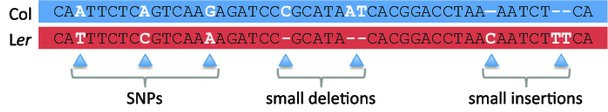
\includegraphics[width=0.8\textwidth,height=\textheight,keepaspectratio]{images/Mec_evo.jpg}
    \caption[Identification des SNP et indels entre 2 génomes]{SNP et InDels entre deux génomes. On suppose que le premier codon commence par le premier nucléotide. Figure extraite et adaptée de \cite{qi_detection_2014}}
    \label{fig:mec_evo}
\end{figure}

\paragraph{Indels: insertion, délétion et pseudogènes}

Un indel correspond à l'insertion (In) ou la délétion (del)\footnote{On regroupe l'insertion et la délétion, car sans une analyse phylogénétique, il est impossible de les différencier par comparaison de séquence.} d'un ou plusieurs nucléotides dans la séquence d'un gène. 

Lorsque la taille de l'indel est un multiple de 3 (insertion ou délétion d'un codon), la séquence protéique peut soit être allongée soit raccourcie d'un acide aminé, soit coupée de façon précoce si le codon est un codon STOP.

Si la taille de l'indel n'est pas un multiple de 3, il y aura un décalage du cadre de lecture ou \textit{frameshift}. Ce décalage va induire un changement de tous les acides aminés de l'indel à la fin du gène, provoquant avec lui un changement dans la fonction de la protéine ou une inactivation de la fonction. La partie du gène qui n'est pas décalée est alors considérée comme un fragment du gène initial, il est alors qualifié de pseudogène. À nouveau, cette mutation peut être délétère pour la cellule. Sur la \autoref{fig:mec_evo}, les Indels sont de taille 1 et 2, elles ne provoquent pas l'apparition d'un codon STOP précoce, mais l'ensemble des acides aminés est modifié.

Les indels vont donc transformer la séquence protéique traduite, pouvant nuire à la fonction de cette dernière et être délétère pour l'organisme. Pour éviter les problèmes liés aux \textit{frameshifts}, il a été montré qu'il existe un fort taux de codon STOP hors du cadre de lecture \cite{tse_natural_2010}. Cette adaptation permettrait de limiter la traduction des protéines mutantes et d'ainsi limiter le coût énergétique pour la cellule. Il a aussi été montré que les \textit{frameshifts} pourraient être à l'origine d'un réservoir d'adaptation à l'environnement \cite{koch_catastrophe_2004}. Lors d'un changement dans l'environnement créant une nouvelle pression de sélection, un \textit{frameshift} pourrait produire une protéine qui permet à l'organisme de s'adapter à son environnement et donc d'améliorer sa \textit{fitness}\footnote{Le \textit{fitness} correspond à la capacité d'un individu de survivre dans son environnement et à se reproduire}. Une fois que l'élément perturbateur de l'environnement disparaît, un nouveau \textit{frameshift} pourrait ramener le cadre de lecture à sa place d'origine. Ce mécanisme, en accord avec la petite taille des génomes, aurait l'intérêt de ne pas perdre des gènes d'adaptation à l'environnement, même s'ils ne sont nécessaires que ponctuellement.

\subsubsection{Réarrangement génomique : un moteur de l'évolution}
\label{sec:rearragement}
Les mécanismes de réarrangement génomique sont très importants dans l'évolution des génomes, mais qui, par rapport aux mutations, impliquent des segments d'ADN plus important. La forme du génome obtenue, appelée un variant structural (SV pour \textit{Structural variant} en anglais), est plus difficile à détecter que les SNP et les indels \cite{periwal_insights_2015}.

Le mécanisme de recombinaison est à l'origine des réarrangements. Une recombinaison implique l'échange de 2 portions d'ADN entre 2 molécules ou 2 régions d'ADN. La recombinaison peut être homologue, se produisant entre des séquences similaires, ou non homologue, impliquant des séquences différentes. Elle est souvent médiée par des enzymes spécialisées comme RecA ou des intégrases, qui permettent l'intégration, la réparation ou le réarrangement précis des séquences. La recombinaison homologue est cruciale pour la réparation des cassures de l'ADN, les réarrangements et également dans l'acquisition de nouveaux gènes par transfert horizontal (cf. \autoref{sec:evo_hz}) \cite{eisenstark_genetic_1977}.

Les réarrangements de l'ADN correspondent donc globalement à un échange entre 2 segments du génome, induisant une insertion, une délétion ou une modification de l'ordre des nucléotides (\autoref{fig:rearrangement}). Les réarrangements sont fréquents dans les génomes procaryotes \cite{sun_genome-wide_2012}. L'ordre des gènes étant important (cf. \autoref{sec:structure_org}) dans l'expression des gènes et la fonction des protéines, le SV résultant peut conduire à une modification de l'expression génique ou un changement dans la fonction de la protéine. Il existe 3 formes de réarrangement : symétrique, asymétrique et au sein d'un réplicon. Ces formes ne sont pas toutes équiprobables, car elles affectent plus ou moins la structure du génome. Aussi, les réarrangements proches de l'Ori sont plus fréquents que ceux proches du site de terminaison \cite{darling_dynamics_2008}. 

\begin{figure}[htbp]
    \centering
    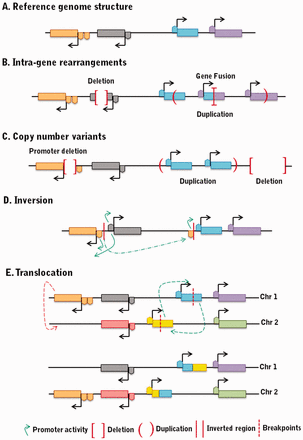
\includegraphics[width=\textwidth,height=0.45\textheight,keepaspectratio]{images/rearrangement.png}
    \caption[Réarrangement et implication]{Réarrangement et conséquences des variants structuraux. (A) Région génomique sans SV. Les réctangles représentent les gènes et les petits connecteurs à côté représentent le promoteur du gène concerné. (B) Réarrangement intragénique illustrant la délétion et la fusion de gènes à la suite d'une duplication partielle du gène. Les régions codantes modifiées produisent des transcrits aberrants. La délétion ou la duplication peut entraîner une modification du nombre des gènes dans des régions par ailleurs fonctionnellement intactes. (C) Délétion du promoteur, la régulation est modifiée et une duplication/délétion qui modifie le nombre de copis des gènes. (D) Inversions affectant la structure du gène, le gène est inversé, retourné et réarrangé, ce qui éloigne l'un des promoteurs du premier gène (orange). (E) Translocations affectant le contexte génique. Figure extraite et adaptée de \cite{periwal_insights_2015}}
    \label{fig:rearrangement}
\end{figure}

Les recombinaisons peuvent également mener à la copie de gènes ou de régions génomiques. Cet événement de duplication joue un rôle essentiel dans l'évolution des procaryotes en fournissant une redondance génétique : l'une des copies du gène peut conserver sa fonction d'origine, tandis que l'autre peut accumuler des mutations sans affecter la survie de l'organisme. De plus, la duplication peut également avoir un rôle dans l'expression de gènes spécifiques. C'est le cas des gènes codant pour les pompes à efflux qui évacuent les antibiotiques de l'organisme, qui sont fortement dupliqués \cite{maddamsetti_duplicated_2024}. Dans les génomes, les événements de duplication semblent minoritaires par rapport aux transferts horizontaux \cite{tria_gene_2021}, et ceux en partie dus à l'élimination de la redondance dans les génomes. 

\subsection{Mécanismes d'évolution intragénérationnelle}
\label{sec:evo_hz}

Les mécanismes qui viennent d'être décrits apportent donc de l'innovation dans les génomes procaryotes, ces innovations doivent ensuite être transmises dans la population. Si on ne prend en compte que le transfert vertical, l'innovation ne peut être transmise que d'une génération à une autre, or le temps de génération\footnote{temps nécessaire pour que le nombre de cellules double} peut être relativement long (20 minutes chez \textit{E. coli}, 80 min pour \textit{Lactobacillus acidophilus}\footnote{Bactérie probiotique, elle est utilisée dans la composition de lait fermenté et d'anti-infectieux intestinaux.} et 800 min pour \textit{Mycobacterium tuberculosis}\footnote{Bactérie responsable de la tuberculose chez l'homme, on la retrouve principalement dans les voies respiratoire.}). De plus, un temps de génération plus grand semblerait diminuer le taux de mutation spontanée de l'ADN \cite{weller_generation-time_2015}. Les procaryotes possèdent donc d'autres mécanismes pour échanger de l'ADN avec leur environnement (autres procaryotes de la même espèce ou non, virus, eucaryotes, ADN libre\dots) leur permettant d'intégrer un segment d'ADN contenant une potentielle innovation. Ces mécanismes sont regroupés sous le terme de transfert horizontal. 

\subsubsection{Conjugaison : la sexualité des procaryotes}

La conjugaison a été découverte en 1946 par Joshua Lederberg et Edward L. Tatum \cite{lederberg_sex_1953}, qui décrivent ce mécanisme comme la manière sexuée des bactéries d'échanger de l'ADN. En effet, par analogie, la conjugaison demande un contact direct entre une cellule donneuse et une cellule receveuse pour l'échange de matériel génétique\footnote{N.B : Le transfert est unidirectionnel, la cellule donneuse ne peut recevoir de l'ADN et la receveuse ne peut en donner.}. Il existe 2 catégories d'élément génétique mobile (MGE, pour \textit{Mobile Genetic element} en anglais) conjugatif: les plasmides (cf. \autoref{sec:replicons}) et les éléments intégratif et conjugatifs (ICEs, \textit{Intergrative and Conjugative elements} en anglais). Sur la \autoref{fig:conjugaison} est représenté l'échange d'un plasmide par conjugaison. Les ICEs \cite{johnson_integrative_2015}, contrairement aux plasmides, sont directement intégrés au chromosome, ce qui rend leur réplication dépendante du chromosome, mais qui permet leur transfert de manière verticale aussi. Les ICEs pour être échangé doivent suivre un schéma circulaire : excision du chromosome, circularisation, réplication, transfert et réintégration dans le chromosome. Lors de l'étape d'excision, il peut arriver que des gènes flanquant l'ICEs soit excisé aussi, apportant une nouvelle forme à l'ICE \cite{gibbons_genomic_2011}.

\begin{figure}[htbp]
    \centering
    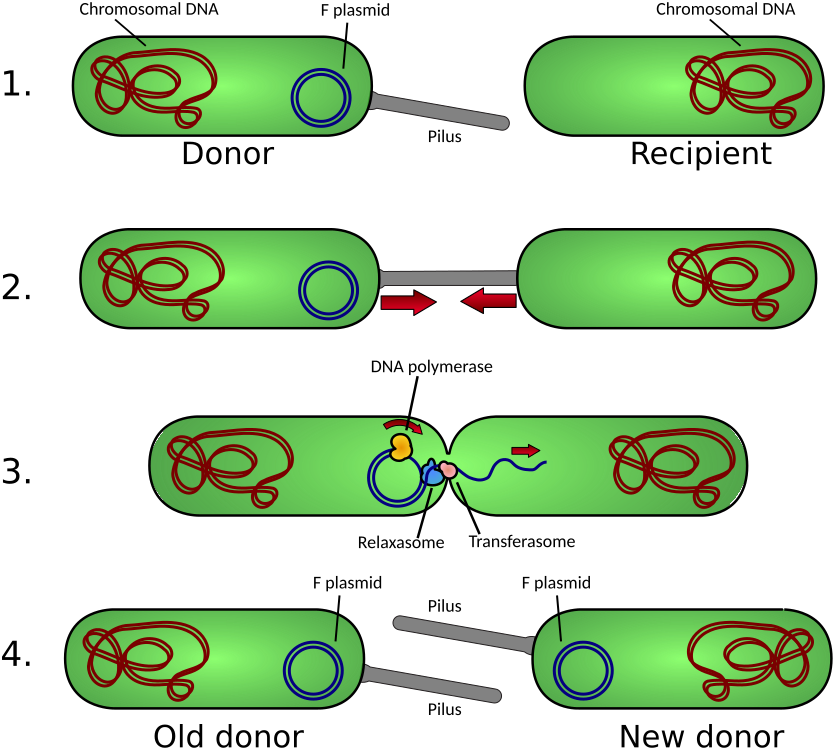
\includegraphics[width=0.8\linewidth]{images/Conjugation.png}
    \caption[Schéma du fonctionnement de la conjugaison]{Schéma du fonctionnement de la conjugaison, dans le cas d'un plasmide conjugatif. (1) Formation d'un pili sexuel par la bactérie donneuse. (2) Contact direct entre les 2 bactéries via le pili. (3) Réplication de l'ADN plasmidique et transfert à la bactérie donneuse. (4) Terminaison de la conjugaison et nouvelle formation d'un pili pour la receveuse devenue donneuse. Image sous licence Creative Commons 3.0 \url{https://commons.wikimedia.org/wiki/File:Conjugation.svg}}
    \label{fig:conjugaison}
\end{figure}

Plasmides et ICEs sont généralement de petite taille, mais ils contiennent des gènes clés d'adaptation aux conditions environnementale. La colocalisation des gènes d'adaptation avec ceux de la conjugaison permet à des colonies de répondre efficacement et rapidement aux nouvelles conditions environnementales, comme la présence de métaux lourds ou d'antibiotique \cite{botelho_role_2021}. Toutefois, tous les MGEs ne sont pas forcément conjugatif \cite{valentine_mobilization_1988}, ils vont profiter de la conjugaison codée par un autre élément pour se transférer. Dans ces conditions, la bactérie receveuse ne devient pas conjugative à son tour, même si elle reçoit l'élément mobile. Ces éléments mobilisables sont appelés des IMEs (élément intégratif mobilisable). Il est d'ailleurs à noter que tous les plasmides ne sont pas mobilisables, il y aurait d'ailleurs autant de plasmide conjugatif que de plasmide non mobilisable \cite{smillie_mobility_2010}.

La conjugaison est un mécanisme majeur de transfert horizontal de matériel génétique, qui a la caractéristique de rapidement répandre les éléments mobiles. Il a toutefois le défaut de limiter le transfert de gènes entre cellule procaryote et donc de limiter le transfert aux innovations génétique déjà intégré par un autre organisme procaryote. Ce n'est pas le cas des prochains mécanismes que nous décrirons.   

\subsubsection{Transformation : recycler l'ADN environnant}

La transformation correspond à l'intégration d'un fragment d'ADN étranger dans le génome de l'organisme. Ce qui  différencie la transformation de la conjugaison, c'est que l'ADN intégré est libre dans l'environnement
\footnote{La découverte de la transformation en 1928 par Fred Griffith \cite{griffith_significance_1928}, précède de nombreuses années celle qui a mis en évidence que l'ADN est le porteur de l'information génétique \cite{avery_studies_1944}. La transformation est donc une preuve anticipée et un socle pour démontrer le rôle de l'ADN.}. Bien que la transformation soit un processus répandu chez les bactéries, elles n'en sont pas toutes capables. Les bactéries pouvant réaliser la transformation sont dites compétentes. De plus, même si les mécanismes de la transformation sont bien décrits \cite{johnston_bacterial_2014,dubnau_mechanisms_2019}, notamment sur l'incorporation de l'ADN dans la cellule (\autoref{fig:transformation}), d'une espèce procaryote à l'autre, ils peuvent varier tout comme la proportion de transformation réalisée \cite{stewart_biology_1986}. Nous ne reviendrons donc pas sur les mécanismes, mais seulement sur des exemples d'application.

\begin{figure}[htbp]
    \centering
    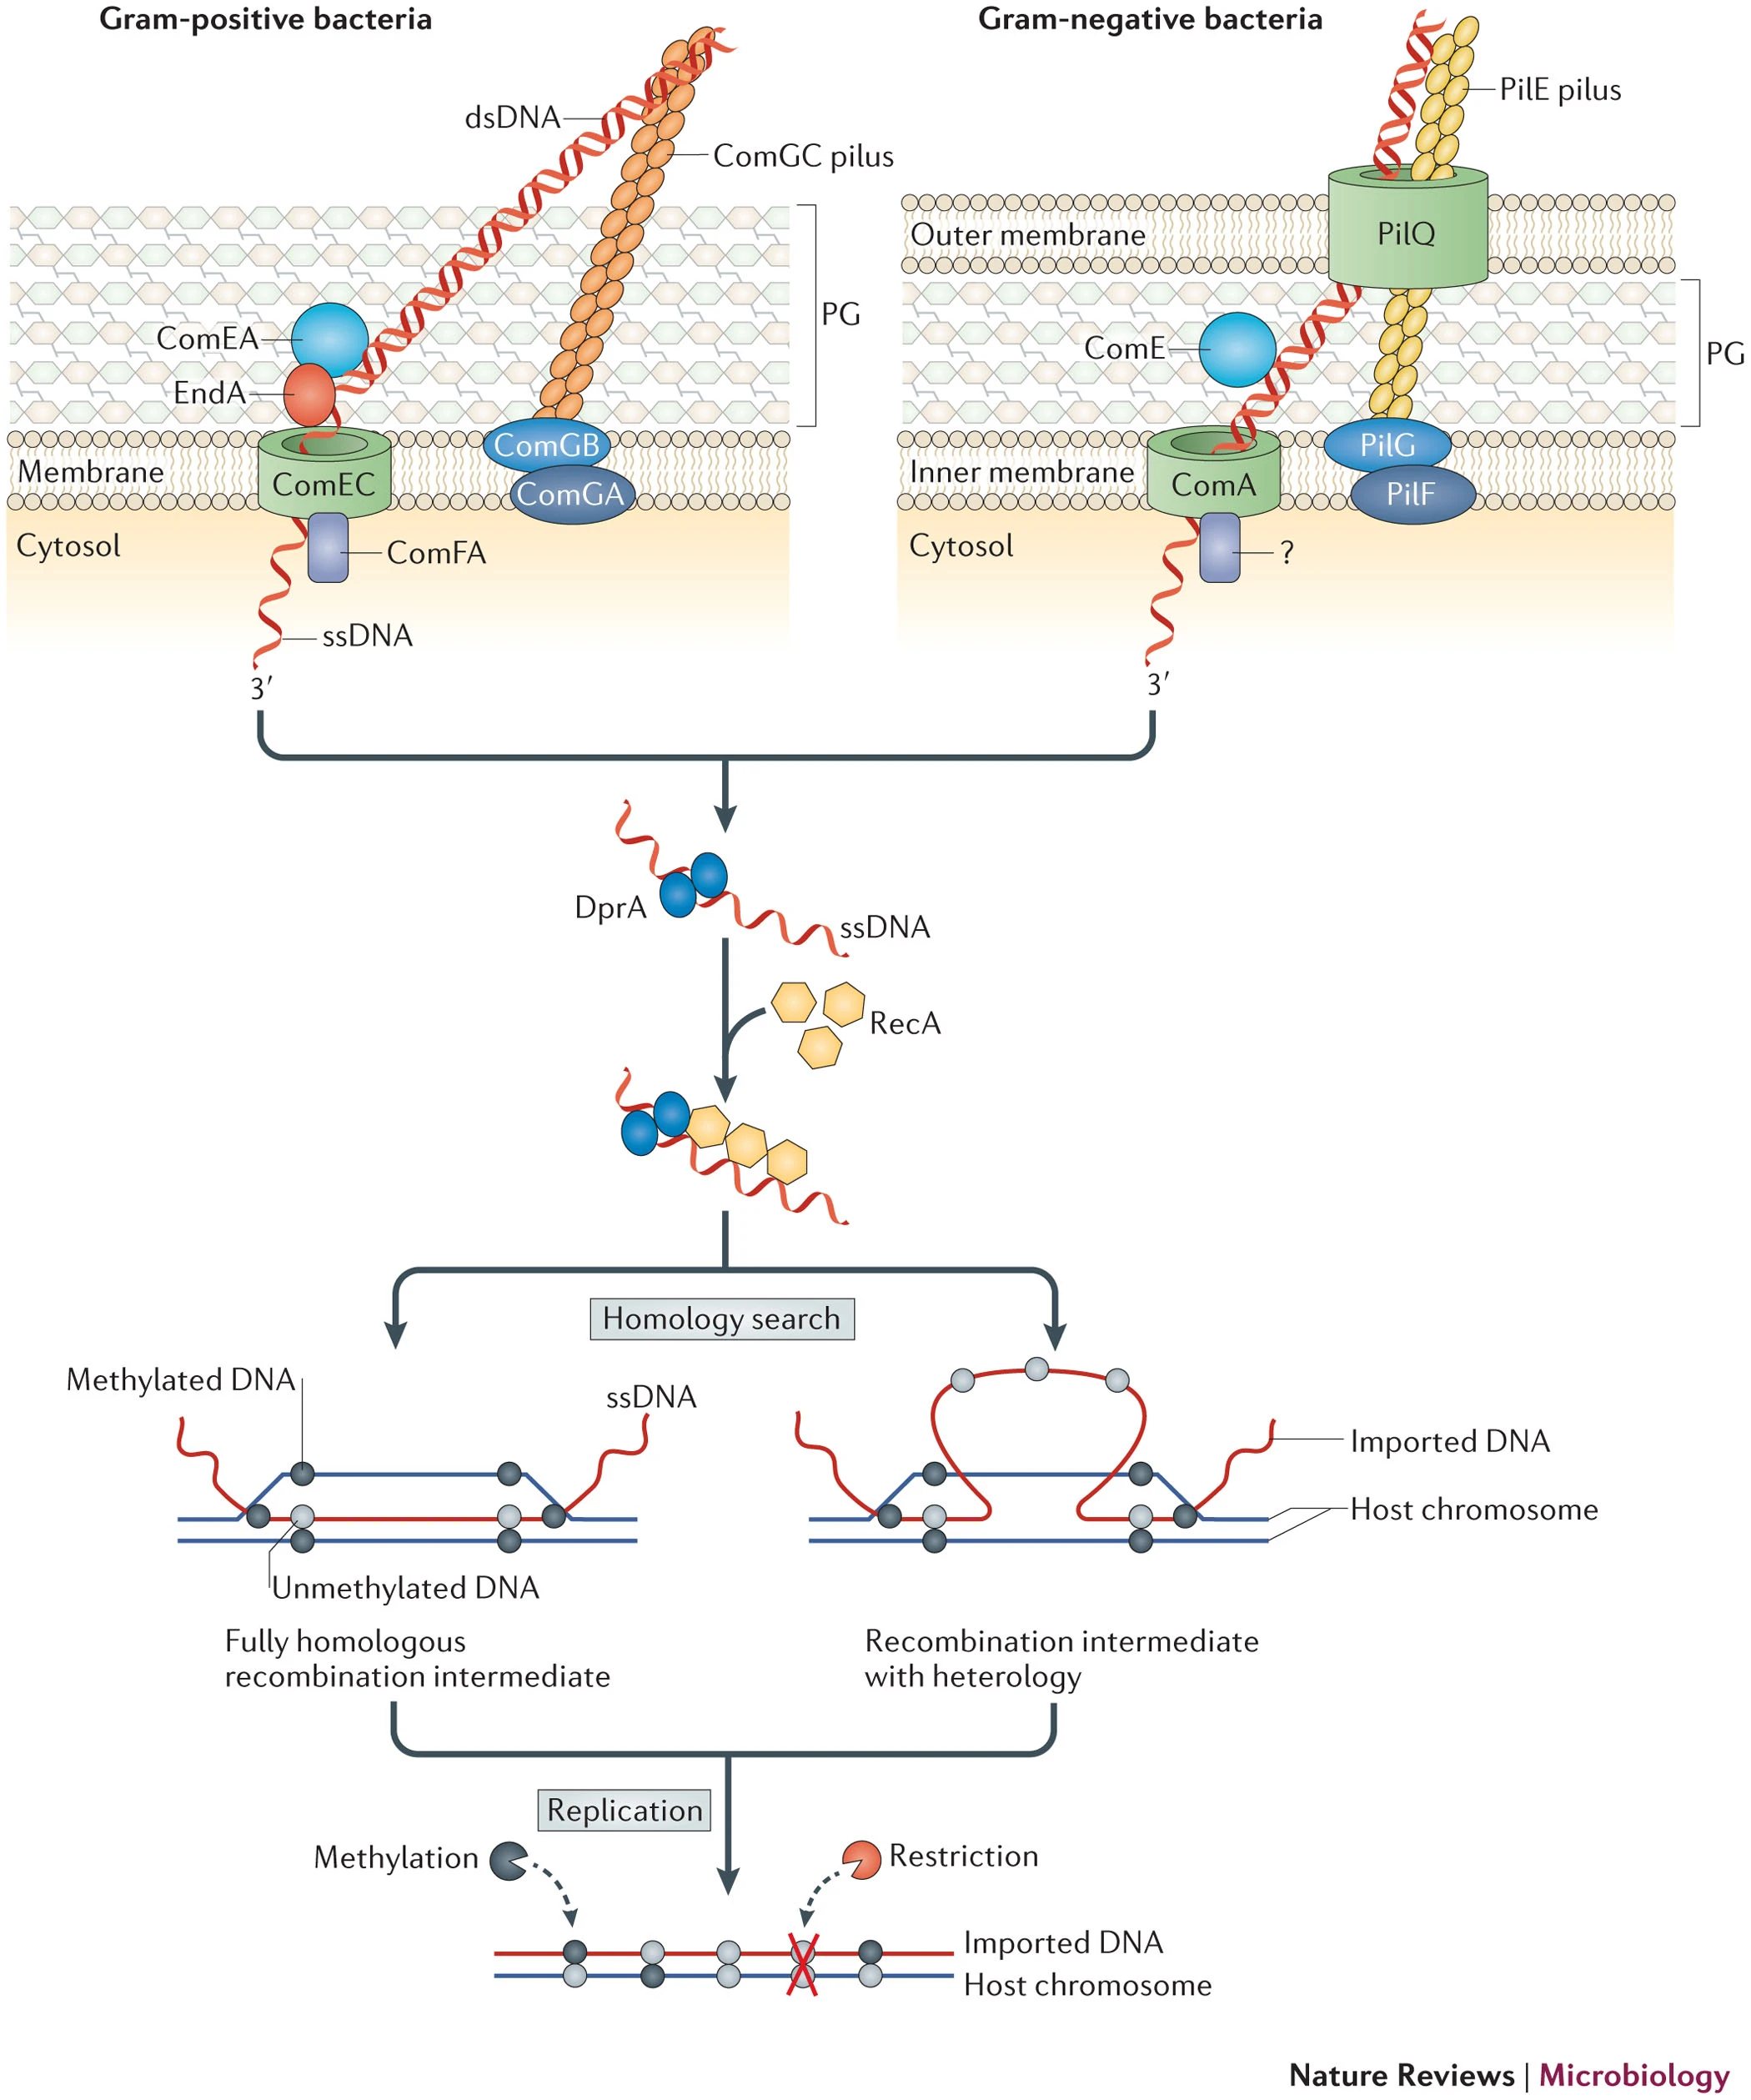
\includegraphics[width=0.8\linewidth]{images/transformation.png}
    \caption[Schéma du mécanisme de transformation]{Schéma du mécanisme de transformation. Extrait de \cite{johnston_bacterial_2014}}
    \label{fig:transformation}
\end{figure}

Les bactéries du genre \textit{Nesseria} et particulièrement \textit{N. gonorrhoeae}\footnote{Ce genre bactérien vit dans les muqueuses des mammifères et est non pathogène à l'exception de \textit{N. meningitidis}, impliqué dans la méningite et \textit{N. gonorrhoeae}, responsable de la gonorrhée, une infection sexuellement transmissible.} reconnaissent préférentiellement une séquence d'ADN non palindromique de leur propre ADN \cite{goodman_identification_1988,duffin_dna_2010}. Ce système permet d'intégrer uniquement l'ADN de souche proche, ainsi des gènes d'adaptation, comme de résistance aux antibiotiques \cite{centers_for_disease_control_and_prevention_cdc_update_2007}, sont distribués préférentiellement dans l'espèce.

Les \textit{Streptococcus pneumoniae}\footnote{Bactérie connue pour son rôle d'agent pathogène dans les pneumonies et responsable de co-infection pendant la grippe espagnole} utilise la transformation comme mécanisme de réparation de l'ADN, car cette espèce ne possède pas de système de réparation SOS. Les \textit{S. pneumoniae} s'engagent alors dans une "guerre fratricide" pour récupérer l'ADN de son espèce.

Pour terminer, chez \textit{Bacillus subtilis}\footnote{Bactérie du sol, mais qu'on retrouve dans de nombreux habitat dû à ses capacités d'adaptation. Elle est utilisé comme modèle d'étude des bactérie Gram+.}, la transformation entre individus de la même espèce, mais de souche éloignée, est privilégiée \cite{lyons_combinatorial_2016}. Les bactéries vont sécréter dans l'environnement des antibiotiques, auxquels elles sont résistantes, pour tuer les autres individus de l'espèce. L'ADN récupéré est donc différent de celui de la bactérie et donc potentiellement source de nouvelles fonctions.

Ces exemples montrent aussi une opposition dans la philosophie des mécanismes de conjugaison et de transformation. La transformation demande que l'ADN soit libre dans l'environnement et donc que les bactéries environnantes soient détruites, alors que la conjugaison laisse les 2 cellules en vie. 


\subsubsection{Transduction : les virus mis à profit}

La transduction est un mécanisme reposant sur l'intervention d'un virus pour transporter et transférer le matériel génétique d'une cellule procaryote à l'autre (\autoref{fig:transduction}). Les virus de bactéries, surnommés (bacterio)phages\footnote{Officiellement bactériophage, mais raccourci dans l'usage en phage}, vont infecter la cellule donneuse pour répliquer leur ADN. Lors de la réplication, de l'ADN de la cellule donneuse peut se trouver intégré à celui du phage. Lorsqu'il infectera une cellule receveuse, la portion d'ADN de la donneuse pourra reprendre une forme plasmidique (si c'est un plasmide qui a été transféré) ou être intégrée au génome de la cellule par recombinaison homologue. La transduction est aujourd'hui largement utilisée en génétique et microbiologie pour transférer de l'ADN et modifier les génomes \cite{wang_phage-based_2024}. 

\begin{figure}[htbp]
    \centering
    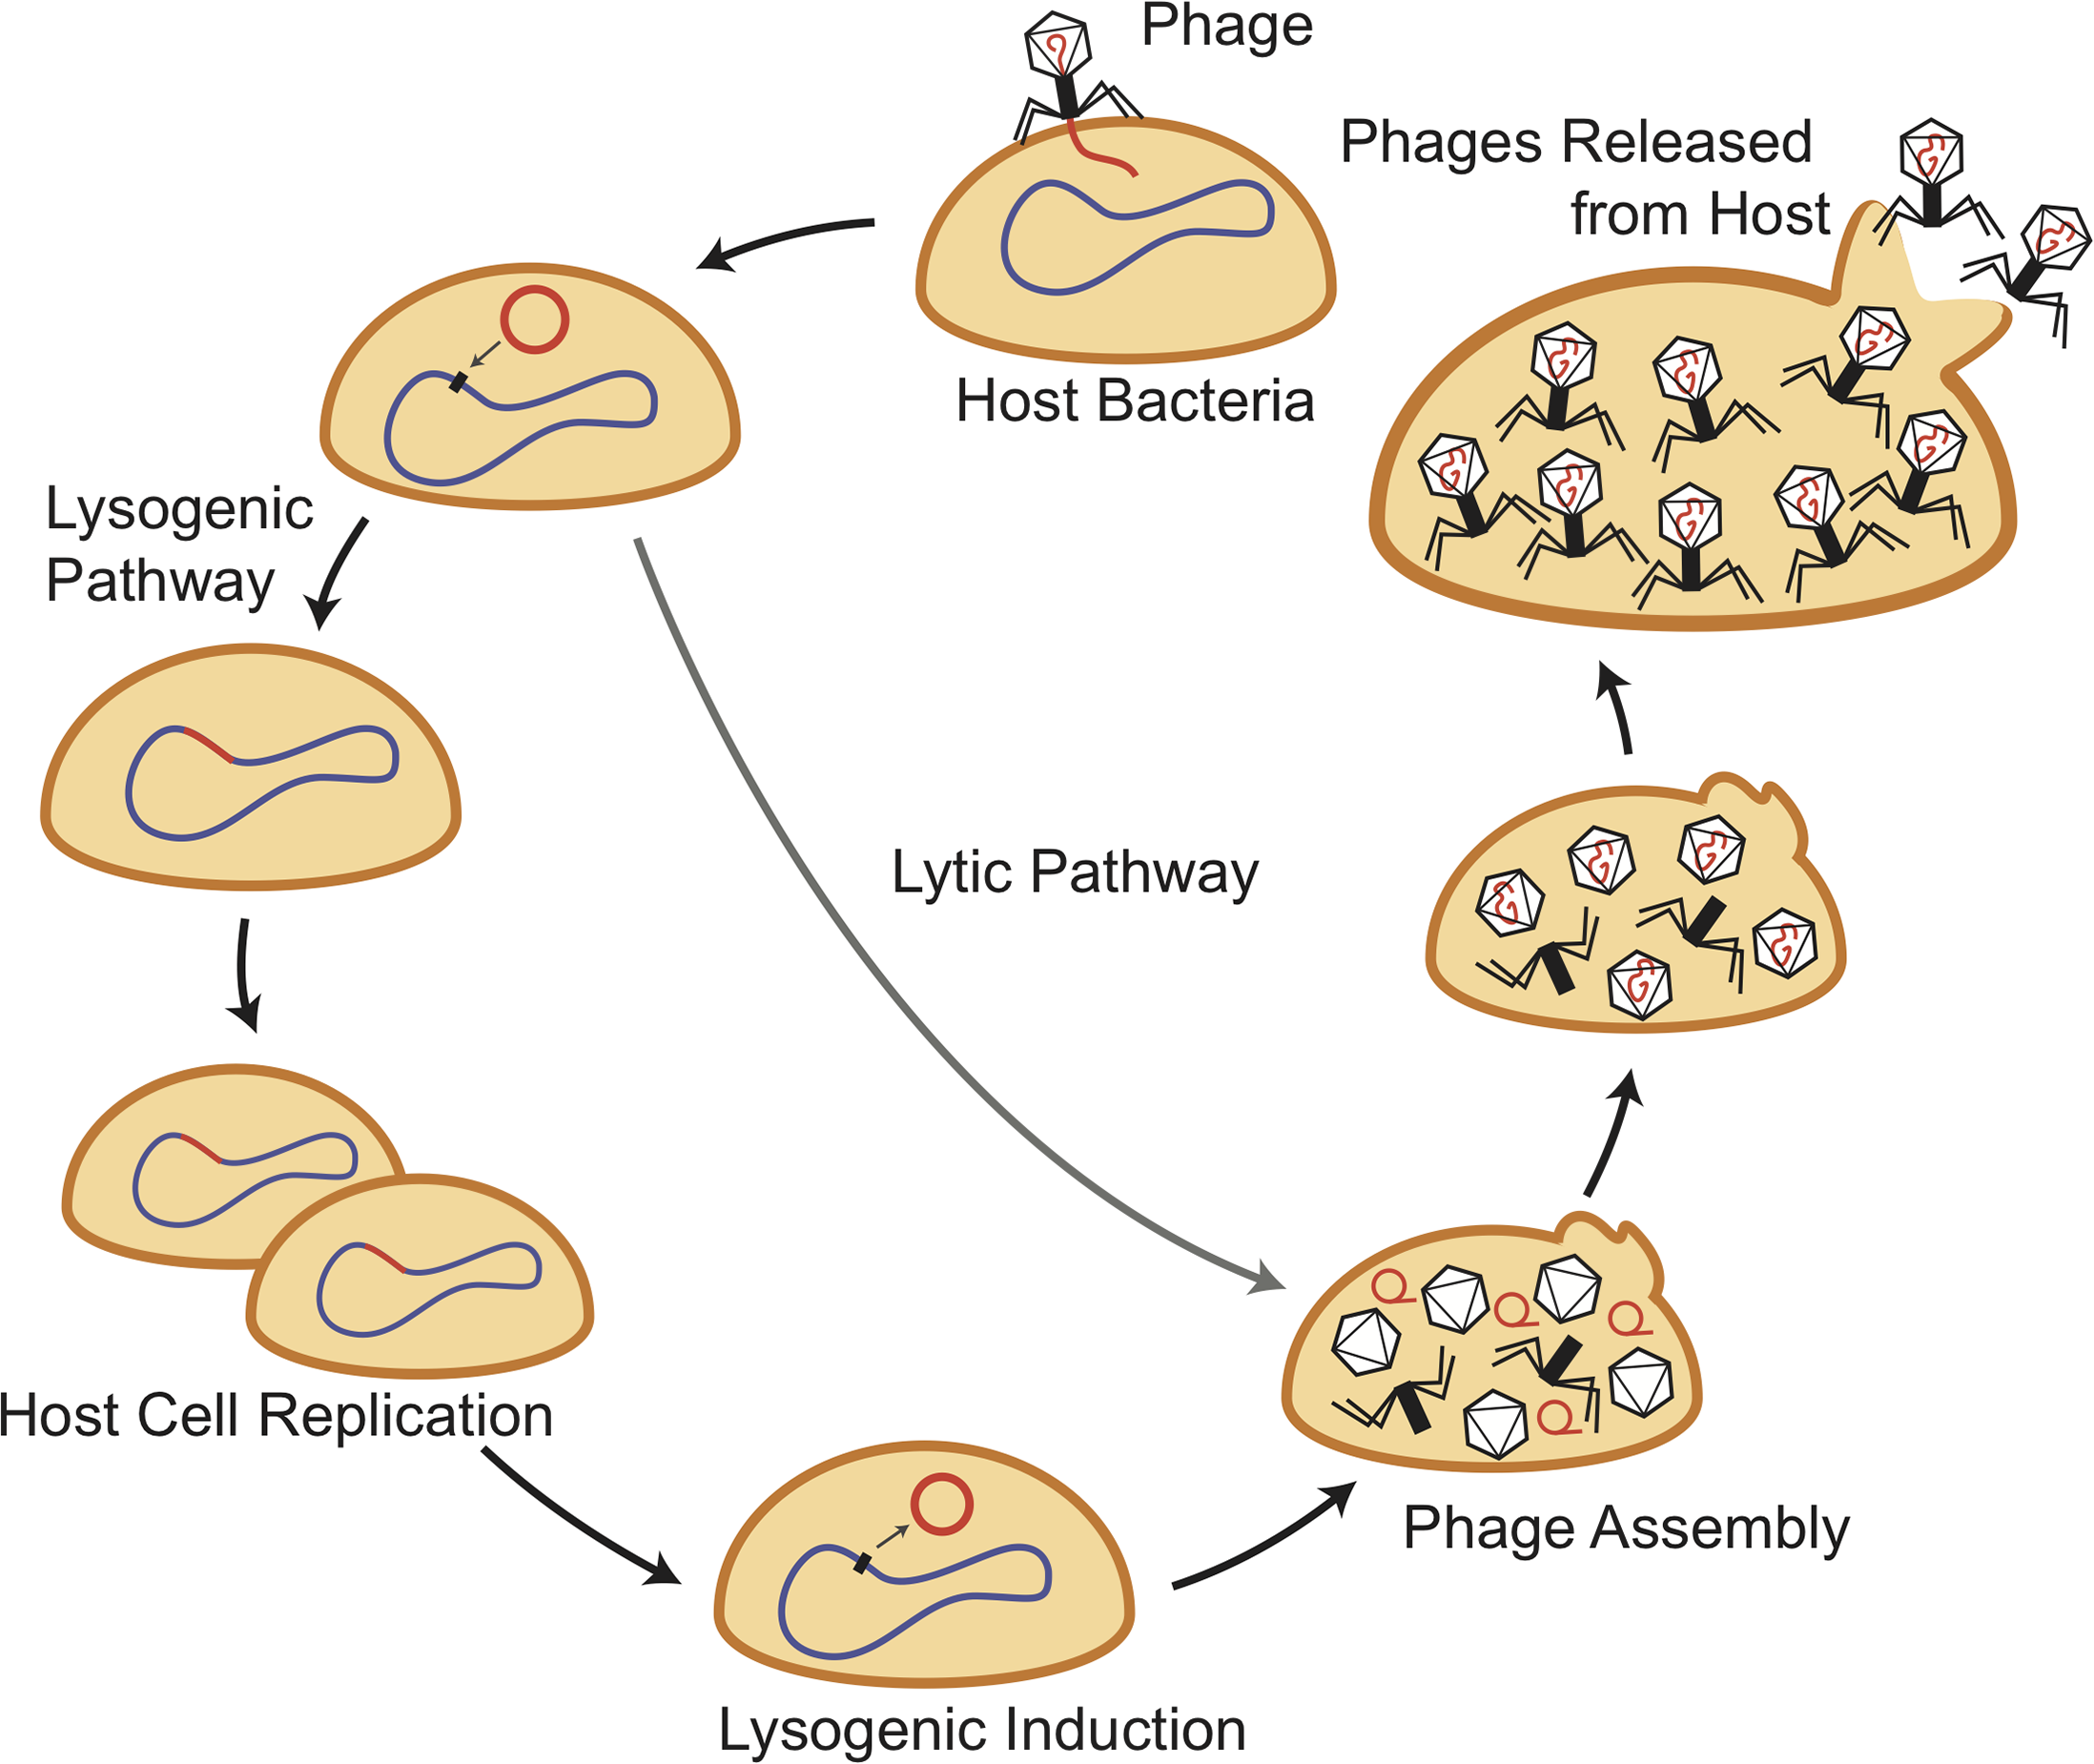
\includegraphics[width=0.65\linewidth]{images/transduction.png}
    \caption[Schéma synthétique de la transduction]{Schéma représentant les étapes de transduction. Extrait de \cite{chiang_genetic_2019}}
    \label{fig:transduction}
\end{figure}

La première forme de transduction identifiée décrivait le transfert de n'importe quel gène de la donneuse à la receveuse par le phage. Cette forme a donc été nommé transduction généralisée \cite{zinder_genetic_1952}. Une seconde forme dites spécifique a été découverte en étudiant le phage $\lambda$ infectant les \textit{E. coli} \cite{morse_transduction_1956}. Le transfert se limite à un ensemble de gènes définis. Enfin, une dernière forme, la transduction latérale, a récemment été découverte \cite{chen_genome_2018}. Là où les formes générale et spécifique peuvent être vues comme une erreur et un évènement lié au hasard, la transduction latérale fait partie du cycle de vie du phage, menant à un taux de transfert beaucoup plus important. 